\documentclass[12pt]{extarticle}
%Some packages I commonly use.
\usepackage[english]{babel}
\usepackage{graphicx}
\usepackage{framed}
\usepackage[normalem]{ulem}
\usepackage{amsmath}
\usepackage{amsthm}
\usepackage{amssymb}
\usepackage{amsfonts}
\usepackage{enumerate}
\usepackage[utf8]{inputenc}
\usepackage[top=1 in,bottom=1in, left=1 in, right=1 in]{geometry}
\usepackage{url}
\usepackage{fancyhdr}
\usepackage{listings}
\usepackage{xcolor}
\usepackage{afterpage}
\definecolor{codegreen}{rgb}{0,0.6,0}
\definecolor{codegray}{rgb}{0.5,0.5,0.5}
\definecolor{codepurple}{rgb}{0.58,0,0.82}
\definecolor{backcolour}{rgb}{0.95,0.95,0.92}
\lstset{ 
	language=Matlab,                		% choose the language of the code
	backgroundcolor=\color{backcolour},   
    commentstyle=\color{codegreen},
    keywordstyle=\color{magenta},
    numberstyle=\tiny\color{codegray},
    stringstyle=\color{codepurple},
    basicstyle=\ttfamily\footnotesize,
    breakatwhitespace=false,         
    breaklines=true,                 
    captionpos=b,                    
    keepspaces=true,                 
    numbers=left,                    
    numbersep=5pt,                  
    showspaces=false,                
    showstringspaces=false,
    showtabs=false,                  
    tabsize=2
}


%A bunch of definitions that make my life easier
\newcommand{\matlab}{{\sc Matlab} }
\newcommand{\cvec}[1]{{\mathbf #1}}
\newcommand{\rvec}[1]{\vec{\mathbf #1}}
\newcommand{\ihat}{\hat{\textbf{\i}}}
\newcommand{\jhat}{\hat{\textbf{\j}}}
\newcommand{\khat}{\hat{\textbf{k}}}
\newcommand{\minor}{{\rm minor}}
\newcommand{\trace}{{\rm trace}}
\newcommand{\spn}{{\rm Span}}
\newcommand{\rem}{{\rm rem}}
\newcommand{\ran}{{\rm range}}
\newcommand{\range}{{\rm range}}
\newcommand{\mdiv}{{\rm div}}
\newcommand{\proj}{{\rm proj}}
\newcommand{\R}{\mathbb{R}}
\newcommand{\N}{\mathbb{N}}
\newcommand{\Q}{\mathbb{Q}}
\newcommand{\Z}{\mathbb{Z}}
\newcommand{\<}{\langle}
\renewcommand{\>}{\rangle}
\renewcommand{\emptyset}{\varnothing}
\newcommand{\attn}[1]{\textbf{#1}}
\theoremstyle{definition}
\newtheorem{theorem}{Theorem}
\newtheorem{corollary}{Corollary}
\newtheorem{lemma}{Lemma}
\newtheorem*{definition}{Definition}
\newtheorem*{example}{Example}
\newtheorem*{note}{Note}
\newtheorem{exercise}{Exercise}
\newcommand{\bproof}{\bigskip {\bf Proof. }}
\newcommand{\eproof}{\hfill\qedsymbol}
\newcommand{\Disp}{\displaystyle}
\newcommand{\qe}{\hfill\(\bigtriangledown\)}
\newcommand{\norm}[1]{\left\lVert#1\right\rVert}
\setlength{\columnseprule}{1 pt}
\pagestyle{fancy}
% \fancyhf{}
\rhead{Yusi Chen}
\lhead{ECE 273\quad Project}


\title{Robust PCA and human brain connectivity}
\author{Yusi Chen; A53240542}
\date{\today}

\begin{document}

\maketitle

\tableofcontents

\section{Goal of the project:}
This project focuses on robust PCA, a matrix decomposition problem which aims to separate a matrix into a low rank matrix and a sparse matrix. Candes et al \cite{candes2011robust} proved that this problem can be conveniently solved by a principal pursuit program (PCP). Based on the above paper, the specific goals are stated as follow: 
\begin{itemize}
    \item Understand why PCP can be applied to decompose a matrix and list the main assumptions.
    \item Implement the algorithm as stated in the paper and reproduce the numerical experiments in the paper.
    \item Apply robust PCA to the brain connectivity matrices estimated from human fMRI recordings. 
\end{itemize}

\section{Background and motivation:}
Real-life datasets (such as images, video clips) lie in a very high-dimensional space and are hard to tackle in their original subspaces. Luckily, most of the datasets have low intrinsic dimensionality, which makes them much more approachable. Methods aiming to find this intrinsic dimensionality could have large impact. \\

Classical PCA is probably the most commonly used dimensionality reduction method. It indeed is a matrix decomposition problem because it seeks the best low rank estimation $\hat{L}$ of the original dataset $M$: 
\begin{equation}
\label{pca}
\min ||M-L||, \quad \text{subject to rank(L)}\leq k     
\end{equation}
However, classical PCA assumes the residual matrix $M-L$ to be a small perturbation matrix, as a result, it is susceptible to grossly corrupted observations or outliers. \\

Robust PCA is one of the approaches to save PCA from breaking down under the presence of outliers. It doesn't require the residual matrices to have small values but assume the residual matrix is sparse. The formal expression of the problem would be as follows: 

\noindent Suppose we want to decompose a large data matrix M into a sparse matrix $L_0$ and a low-rank matrix $S_0$.  
\begin{equation}
    M = S_0 + L_0
\end{equation}
Candes et al \cite{candes2011robust} proved that under some suitable assumptions, it is possible to recover both the low-rank and the sparse components \textbf{exactly} by solving a very convenient convex program called Principal Component Pursuit (PCP):
\begin{equation}
    \text{min} \norm{L}_* + \lambda \norm{S}_1, \quad\text{subject to } L+S = M
\end{equation}
In many dimensionality reduction cases, the low rank matrix is the target matrix. But there are also scenarios \cite{yatsenko2015improved} that the sparse matrix becomes the target of interest. Therefore, robust PCA is an algorithm more than just robustifying PCA. \\

The brain connectivity from different human subjects could probably be another dataset that lies in a low dimensional subspace. The basic idea is to stack vectorized brain connectivity of each subject as columns of the big dataset matrix $M$. There is a huge literature \cite{raichle2015brain} showing a common network connectivity mode across subjects. This ensures that there is a low rank component in $M$. The low rank would be 1 if every one has exactly the same connectivity pattern and there is no noise presented. At the mean time, inter-individual variability assures the presence of individual specific connectivity, i.e. the sparse component. In this way, robust PCA can be used to efficiently separate population-level and individual-level network connectivities. But I want to state here that there is no guarantee the low rank and sparsity assumptions hold for the brain connectivity matrices though it is not uncommon for people to apply PCA to connectivity patterns \cite{leonardi2013principal}. It would be still interesting to see the algorithm output.  


\section{Methods}

\subsection{Algorithm}
Following Candes et al \cite{candes2011robust}, I chose the solve the above convex PCP problem using an augmented Lagrange multiplier (ALM) introduced in Lin et al \cite{lin2010augmented}. Briefly, ALM operates on the augmented Lagrangian: 
\begin{equation}
    l(L,S,Y) = ||L||_* + \lambda ||S||_1 + <Y,M-L-S> + \mu/2||M-L-S||_F^2
\end{equation}
A generic Lagrange multiplier would solve the problem by repeatedly solving $(L_k,S_k) = $ argmin $l_{L,S}(L,S,Y)$ and updating $Y_{k+1}=Y_k+\mu(M-L_k-S_k)$. In the case of low-rank and sparse decomposition, the authors suggested to minimize $L$ and $S$ separately because both of these two minimization problems have very simple and efficient solutions. Therefore, the final ALM algorithm is summarized in Figure \ref{alm}. The two element-wise matrix operators are defined as $S_\tau [x] = $sgn$(x)$ max$(|x|-\tau,0)$ and $D_\tau (X) = U S_\tau(\Sigma) V^*$  where $X = U\Sigma V^*$

\begin{figure}
    \centering
    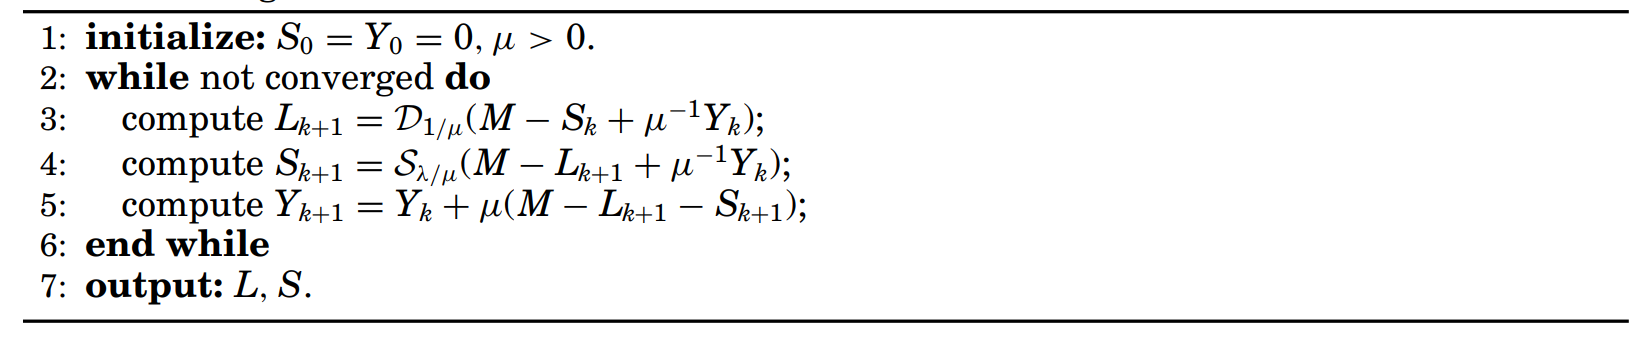
\includegraphics[width=\textwidth]{Screenshot from 2020-06-07 20-12-05.png}
    \caption{ALM algorithm for PCP}
    \label{alm}
\end{figure}

The MATLAB code for implementing ALM could be downloaded from \url{https://people.eecs.berkeley.edu/~yima/matrix-rank/sample_code.html}. 

\subsection{Simulation protocol}
\subsubsection{Random matrices simulation}
Grossly corrupted random matrices $M=L_0+S_0$ of size $N\times N$ were simulated.  The low rank(r) matrix $L_0$ was simulated as $XX^*$ where X is an $n \times r$ i.i.d. long matrix sampled from $\mathcal{N}(0,1/n)$. The support set $\Omega$ of the sparse matrix $S_0$ was uniformly sampled from all the positions and the sign of nonzero entries were independently sampled from a symmetric Bernoulli distribution. A harder decomposition scenario called coherent signals was also simulated. The sign of nonzero entries in $S_0$ is the same to the sign of $L_0$ at the position. That is to say, $S_0$ is the projection of sgn($L_0$) onto the space of the support set matrices. Recovery error was defined as $e = ||\hat{L}-L_0||_F/||L_0||_F$. A trial is considered successful recovery if $e<0.01$.

\subsubsection{Connectivity simulation}
At first, connectivity pattern was directly simulated and corrupted by sparse noise. In this case, the low rank matrix would be one vectorized connection pattern repeated for $N$ times along the column dimension. \\
The second stage is to simulate time series data from the corrupted connectivity pattern $G$ from a simple linear dynamic model. Estimate the covariance matrix from simulated time series data and then apply robust PCA to the stacked big matrix. But I failed to simulate the time series and the possible reasons will be discussed later.
\begin{equation}
\label{dcm}
    \dot{z} = Gz+u,\quad u \sim \mathcal{N}(0,1)
\end{equation}

\subsection{Resting state fMRI dataset pre-processing}
I downloaded the human resting state fMRI dataset from Human Connectome Project (HCP) (\url{https://www.humanconnectome.org/study/hcp-young-adult}). I used the the extensively processed ``HCP1200 Parcellation + Timeseries + Netmats (1003 Subjects)'' dataset. This release included recordings from 1003 healthy adult human subjects (ages 22-37 years, 534 females). The dataset was pre-processed according to Smith et al \cite{smith2013resting}. \\
After pre-processing, the dataset consists of time series data of activity from different brain regions. The covariance matrix was used to estimate brain connectivity. $M$ was created by stacking the vectorized covariance matrices as columns and the robust PCA was applied to it to recover the low rank and sparse component. The representative low-rank connectivity pattern was recovered through SVD. When $L = U\Sigma V^*$, the columns of U which associated with the largest singular values would be the most representative connectivity patterns, denoted as the principal components of low rank matrix. \\
To make the connectivity pattern more readable, I assigned the nodes (representing brain regions) into different sub-networks and sort them accordingly. A sub-network usually includes the brain regions that function together, thus they tend to be more correlated by common sense. Therefore, a more interpretable matrix would appear as a block matrix.

\section{Results}

\subsection{Proof architecture}
Though I may not understand all the details in the proof but I briefly summarized the main theorem and the proof architecture to get a favor.

\subsubsection{Main theorem}
\begin{definition}
Incoherence conditions: \\
Denote the SVD decomposition of $L_0$ as $L_0 = U \Sigma V^* = \sum_{i=1}^r \sigma_i u_i v_i^*$, then the incoherence condition with parameter $\mu$ state that: 
\begin{equation}
    \label{incoherence}
    max_i ||U^*e_i||^2 \leq \frac{\mu r}{n_1}, \quad  max_i ||V^*e_i||^2 \leq \frac{\mu r}{n_2}, \quad ||UV^*||_\infty \leq \sqrt{\frac{\mu r}{n_1n_2}}
\end{equation}
\end{definition}


\begin{theorem}
\label{main}
Suppose $L_0$ is $n_1 \times n_2$, ($n_{(1)} = max(n_1,n_2),\quad n_{(2)} = min(n_1,n_2)$), satisfies the incoherence condition with parameter $\mu$ and \textbf{it is not sparse}. Fix any $n_1 \times n_2$ matrix $\Sigma$ of signs. Suppose the support set $\Omega$ of $S_0$ is uniformly distributed among all sets with cardinality $m$ and that sign($S_0$) = $\Sigma$. Then, there is a numerical constant $c$ such aht with probability at least $1-cn_{(1)}^{-10}$ that PCP with $\lambda = 1/\sqrt{n_{(1)}}$ is exact provided that:
\begin{equation}
 rank(L_0) \leq \rho_r n_{(2)}\mu^{-1}(\log n_{(1)})^{-2},\quad m \leq \rho_s n_1 n_2
\end{equation}
\end{theorem}

\subsubsection{Randomness}
Note that in Theorem \ref{main}, the only piece of randomness comes from the location of the nonzero entries of $S_0$ (i.e. $\Omega$ is uniformly sampled from all subsets with cardinality $m$). During the proof, the authors chose to work with a Bernoulli sampled support set that $\Omega \sim Ber(\rho)$. They proved that the Bernoulli model is equivalent to the uniform model. 

In addition, the authors added one element of randomness. In Theorem \ref{main}, the values of nonzero entries are fixed. For the convenience of proof, the authors assumed that the signs of the nonzero entries are symmetric Bernoulli variables. They established that the results for random signs is sufficient to claim a similar results for fixed signs (Paper Theorem 2.3). 


\subsubsection{Proof through dual certificates}
Denote $\mathcal{P}_\Omega$ as the orthogonal projection onto the linear space of matrices supported on $\Omega$. Denote $T$ as the linear space of matrices: $T = \{UX^*+YV^*, X,Y \in \mathbb{R}^{n \times r}\}$. The operator norm $\mathcal{P}_\Omega$ is defined as $||\mathcal{P}_\Omega || = \sup_{||X||_F=1}||\mathcal{P}_\Omega X||_F$. \\

The authors first proved a dual certificate for $(L_0,S_0)$ to be the unique optimal solution to PCP: 
\begin{lemma}
(Paper Lemma 2.5) Assume $||\mathcal{P}_\Omega \mathcal{P}_T|| < 1/2$ and $\lambda<1$. Then $(L_0,S_0)$ is the unique solution if there exists $W$ obeying: 
\begin{equation}
\label{dual}
\begin{split}
    & W \in T^\perp \\
    & ||W|| < 1/2 \\
    & ||\mathcal{P}_\Omega(UV^* - \lambda sgn(S_0) +W)||_F  \leq \lambda/4 \\
    & ||\mathcal{P}_\Omega^\perp (UV^*+W)||_\infty  \leq \lambda/2
\end{split}
\end{equation}
\end{lemma}
Next, the authors constructed a matrix $W = W^L + W^S$, where $W^L$ is constructed via the golfing scheme and $W^S$ is constructed via the method of least squares. Of note, the construction process requires $L_0$, $S_0$ and $\rho$. Finally, the authors showed that under the assumptions described in Theorem \ref{main}, such $W$ constructed above satisfies Equation \ref{dual} (Paper Lemma 2.8 and 2.9). Therefore, the target low rank matrix $L_0$ and sparse matrix $S_0$ is the unique optimal solution of the PCP problem. 


\subsection{Numerical Experiments}
An example matrix decomposition case is shown in Figure \ref{ex}. Note that in this example, the sparse signal has much higher magnitude compared to the low rank matrix but the algorithm can still successfully recover the original block pattern. This means robust PCA only cares about the matrix structure instead of the matrix values. The ALM algorithm scales up very well from Figure \ref{dim}. The running time was less than 1 seconds on a 8-core computer for all the sizes. In the algorithm, the step of SVD is usually the rate-limiting step. The algorithm usually takes less than 20 SVD steps to converge. \\

Next I tested the algorithm performance using different sparsity values and rank numbers. For each pair, 10 random trials were simulated and the success rate was plotted in Figure \ref{trans}. For the coherent signal, one would expect that the success rate would drop since the sign of nonzero entries of $S_0$ is the same to that of $L_0$. But actually it relaxed the requirement for rank number when the sparsity level is high.  \\



\begin{figure}
    \centering
    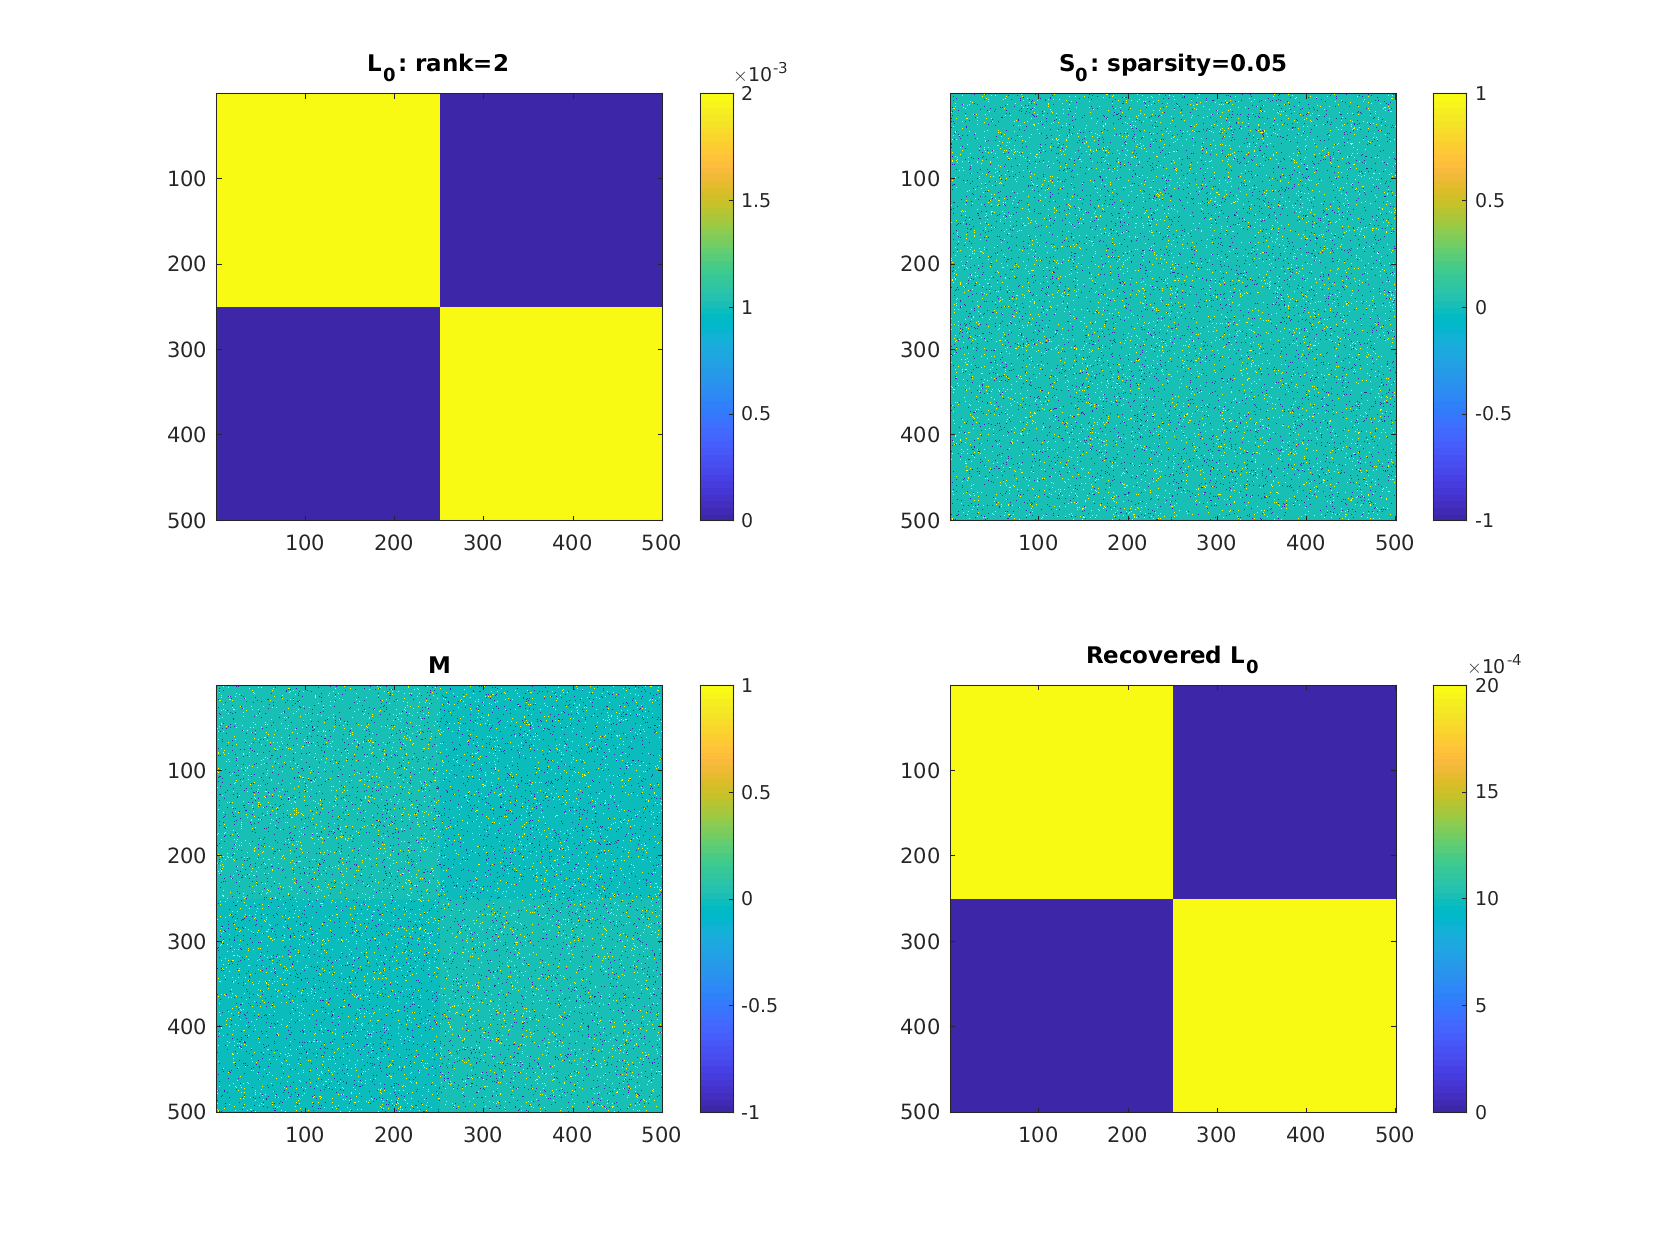
\includegraphics[width=\textwidth]{PatternCorrupted.png}
    \caption{An example of matrix decomposition}
    \label{ex}
\end{figure}

\begin{figure}
\centering
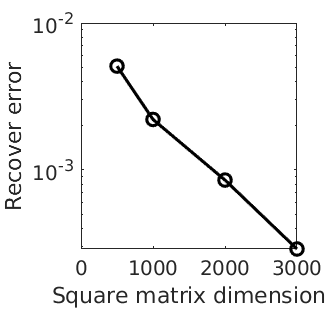
\includegraphics[width=0.3\linewidth]{Error_dim.png}
\caption{Low rank matrix recovery error with matrix dimension}
\label{dim}
\end{figure}

\begin{figure}
    \label{trans}
    \centering
    \begin{minipage}{0.45\textwidth}
    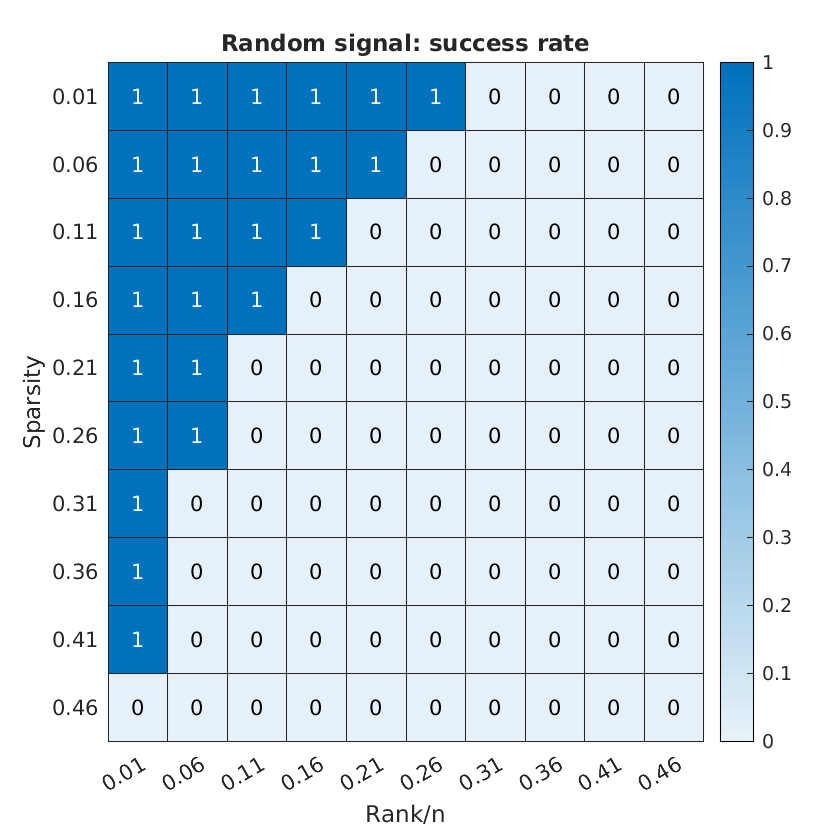
\includegraphics[width=\linewidth]{Random_TransitionPlot.png}
    \end{minipage} \begin{minipage}{0.45\textwidth}
    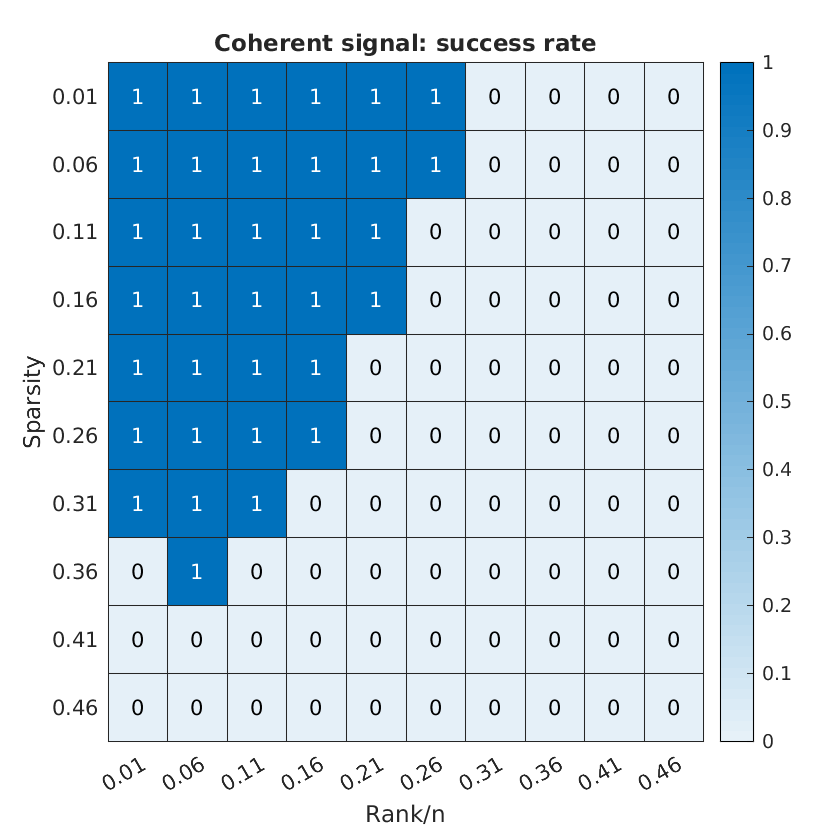
\includegraphics[width=\linewidth]{Coherent_TransitionPlot.png}
    \end{minipage}
    \caption{Success recovery rate of random (coherent) square matrices ($N=500$)}
\end{figure}


\subsection{Application to brain connectivity decomposition}
Two example subject brain connectivity patterns and their decomposition results were shown in Figure \ref{ex_HCP}. Indeed, the low rank component is more consistent despite of the difference in the original covariance matrix. I also plotted the PC1 of low rank matrix compared with the average covariance matrix in Figure \ref{pc}. It seems that the PC1 of the low rank matrix has more visually apparent block structure compared to simply averaging all the matrices. But whether the connectivity pattern presented in PC1 has any biological meaning needs further investigation. Also note that for the two matrices in Figure \ref{pc}, the sign is flipped for some of the block components. The reason for the flipped sign also need further investigation.  

\begin{figure}
    \centering
    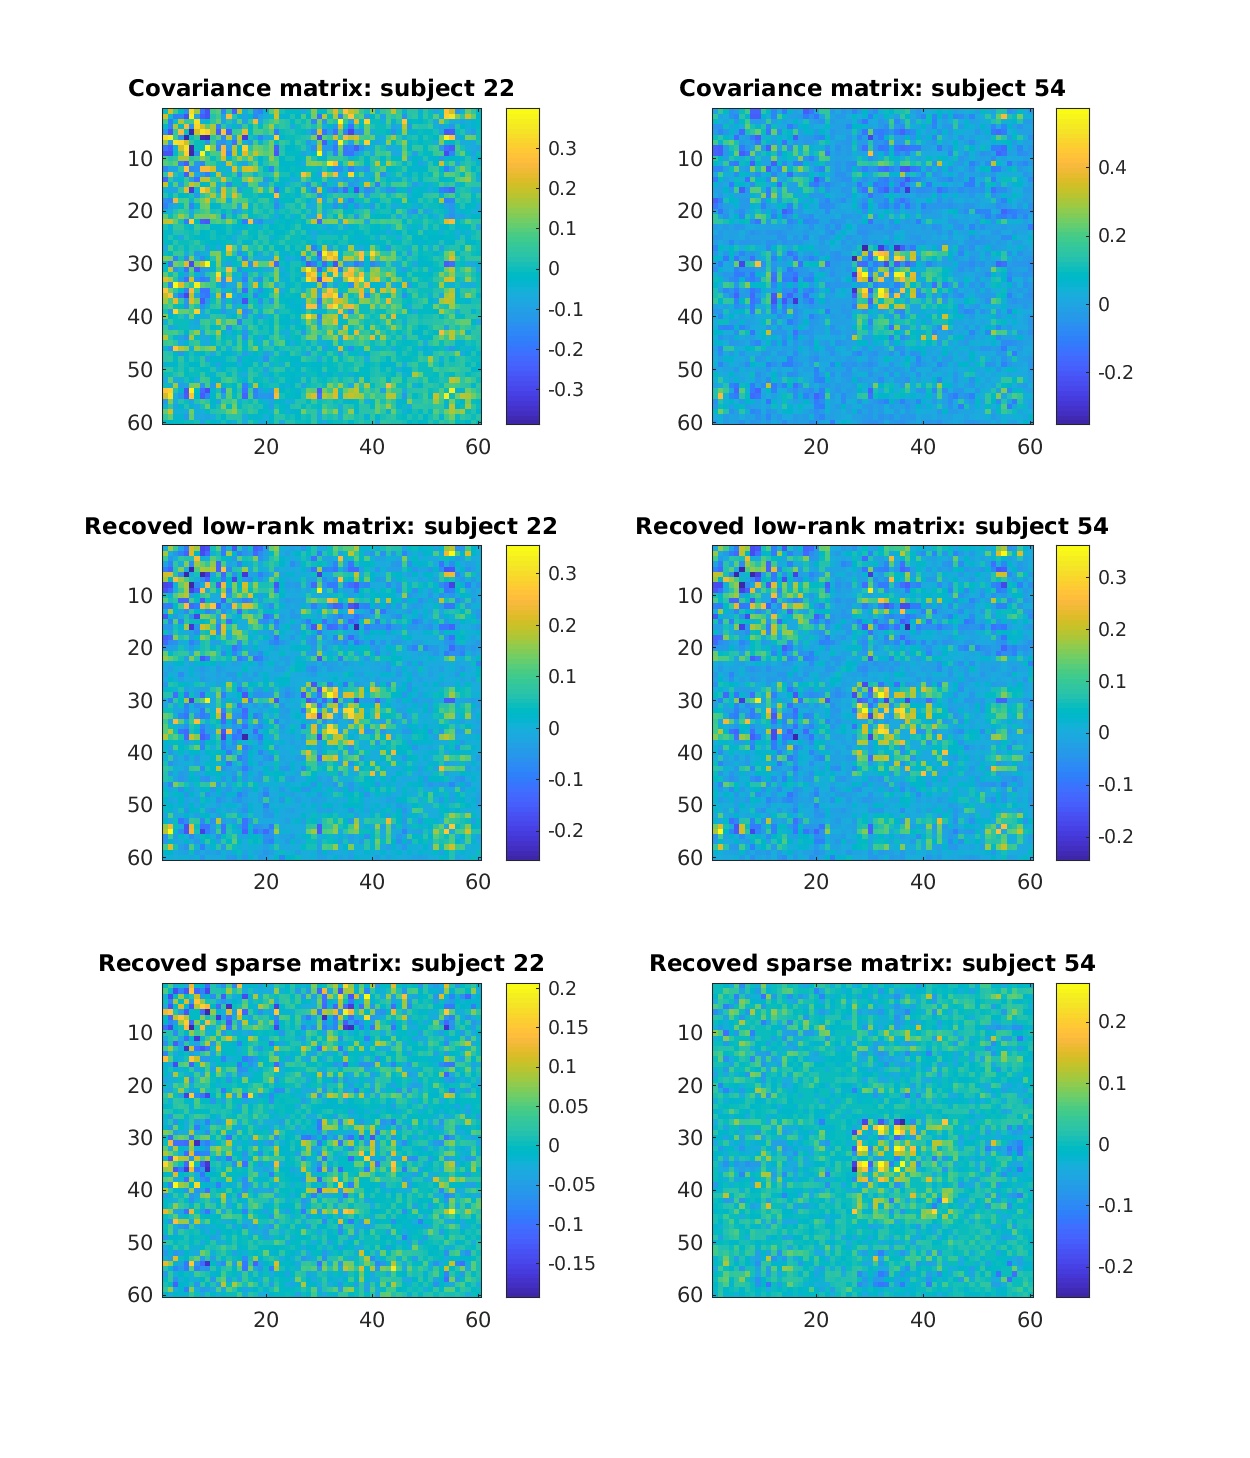
\includegraphics[width=\textwidth]{Example_HCP.png}
    \caption{First row: covariance matrix of two randomly selected subjects; Second row: the recovered low rank matrix; Third row: the sparse matrix}
    \label{ex_HCP}
\end{figure}

\begin{figure}
    \centering
    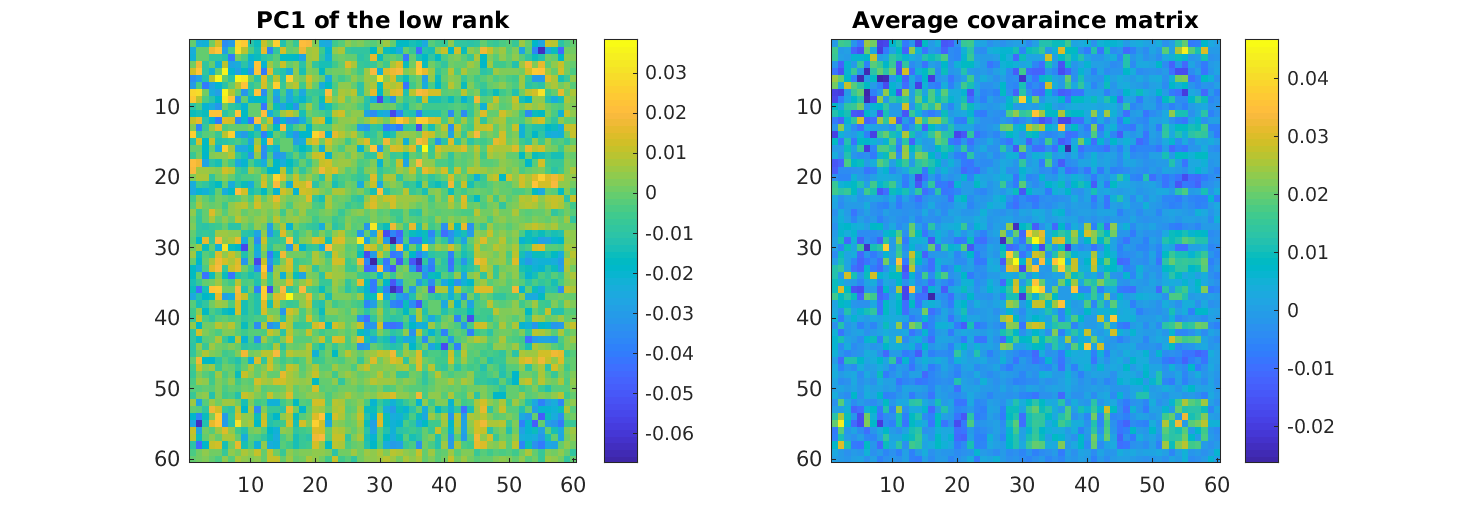
\includegraphics[width=\textwidth]{PC_Avg_HCP.png}
    \caption{Left: first principle component of the recovered low rank matrix; Right: average covariance matrix from 1003 subjects}
    \label{pc}
\end{figure}


\section{Discussion}
Robust PCA implemented by ALM is a very efficient and robust method to decompose matrix. The only assumptions are incoherence condition, rank number and sparsity of its component. All of the three are not hard to satisfied at all (Figure \ref{trans}). But it still remains hard to check the assumptions when applied to real life datasets because the threshold parameters $\mu$, $\rho_s$ and $\rho_L$ remains to be an arbitrary number during the derivation (i.e. the explicit value is not given). It is very robust because the values in $S_0$ can be very large compared to $L_0$ values (Figure \ref{ex}), which is very useful when dealing with grossly corrupted (or missing) datasets. There is also no parameter tuning process since the only parameter $\lambda = 1/\sqrt{N}$. Actually, as long as $\lambda$ lies in a certain range, the PCP optimal pair is always to exact solution to the decomposition problem. On the other hand, since there's no parameter tuning, the decomposition results cannot be tuned towards certain problems. \\

When working on this project, I tried to simulate time series from randomly corrupted connectivity pattern using the simple linear dynamic system as suggested in Equation \ref{dcm}. If this simulation works, the validity of connectivity separation using robust PCA could be better justified. I failed to simulate for long enough time without exploding. For a perfect linear dynamic system $\dot{z} = Az$, as long as the real parts of the eigenvalues of A is non-positive, the system will be explode. Following this, my connectivity matrix was designed as a lower triangular matrix with diagonal values equal to -1. Such matrices have eigenvalues equal to -1. In theory, the dynamic system should not explode. But still, the simulation exploded. The possible reasons could be the randomness term $u$ or the randomly added corrupted connections. \\

In terms of interpreting the low-rank connectivity pattern shown in Figure \ref{pc}, it would be helpful if I could check the biological meanings of the connections found in the PC1 matrix but this is out of the scope of this project. In addition, I think it would be interesting to look at the matrix distance of the low-rank and sparse components between subjects. 

\newpage

\bibliographystyle{plain} 
\bibliography{ref} 

\section{code}
\lstinputlisting[language=Matlab]{Main.m}
\lstinputlisting[language=Matlab]{RandSL.m}
\lstinputlisting[language=Matlab]{inexact_alm_rpca.m}


\end{document}
